% Generated from paper_v7.md; original Markdown is unchanged.
\documentclass{article}
% Anonymous workshop submission. Do not use final or preprint for review.
\PassOptionsToPackage{numbers,sort&compress}{natbib}
\usepackage[dblblindworkshop]{neurips_2026}
\workshoptitle{Physical World AI: Geometry, Characteristics, and Multimodal Sensing}
\usepackage[T1]{fontenc}
\usepackage{amsmath,amssymb}
\usepackage{graphicx,booktabs,longtable,array,calc}
\usepackage{microtype,xcolor,newunicodechar}
\usepackage{url}
\usepackage[hidelinks,unicode]{hyperref}
\newunicodechar{−}{\ensuremath{-}}
\newunicodechar{±}{\ensuremath{\pm}}
\newunicodechar{×}{\ensuremath{\times}}
\newunicodechar{Δ}{\ensuremath{\Delta}}
\newunicodechar{θ}{\ensuremath{\theta}}
\newunicodechar{φ}{\ensuremath{\phi}}
\newunicodechar{ε}{\ensuremath{\epsilon}}
\newunicodechar{→}{\ensuremath{\rightarrow}}
\newunicodechar{≤}{\ensuremath{\leq}}
\newunicodechar{≥}{\ensuremath{\geq}}
\providecommand{\tightlist}{\setlength{\itemsep}{0pt}\setlength{\parskip}{0pt}}
\providecommand{\pandocbounded}[1]{#1}
\setlength{\emergencystretch}{2em}
\graphicspath{{figures/}{../figures/}}
\hypersetup{pdftitle={Bilateral Geometry for Evaluating Predictive Representations of Human Gait},pdfauthor={Anonymous Author(s)},pdfcreator={LaTeX},pdfsubject={Physical World AI workshop submission}}
\title{Bilateral Geometry for Evaluating Predictive Representations of Human Gait}
\author{Anonymous Author(s)}
\begin{document}
\maketitle
\begin{abstract}
Bilateral body structure offers a concrete way to evaluate predictive representations of human movement. A skeleton has named left--right landmark pairs, reflection has a known action on their coordinates and identities, and a signed comparison of movement on the two sides should reverse with that action. We use this relationship to study a skeleton Joint-Embedding Predictive Architecture trained on pose sequences from gait videos. The evaluation keeps source videos separate, compares trained encoders with matched initial weights, and varies where hidden targets fall across anatomy and time. The predictor learns clip-specific feature correspondence, yet the trained encoders recover the signed movement contrast less well than their initializations under the tested readouts. Motion-sensitive summaries make the contrast more accessible at initialization, whereas motion-weighted and connected-region masks show no advantage over count-matched random masks. Reflection augmentation improves one token-consistency measure without a corresponding gain in observable laterality, and the explicit reflection-loss experiment is kept separate because its evidence is synthetic. Taken together, the experiments use bilateral geometry to evaluate whether a predictive representation retains a physically interpretable movement relation, revealing a gap between feature correspondence and the information needed to recover that relation.
\end{abstract}
\section{Introduction}\label{introduction}

Human gait is a useful setting for evaluating physical representations because its geometry is structured while its motion need not be perfectly symmetric. The skeleton supplies named left--right landmark pairs. Reflecting horizontal coordinates and exchanging those landmark identities defines an exact operation on the representation, even though a person's observed gait may differ between sides. We use the term \emph{bilateral geometry} for this pairing of anatomical correspondence with a known reflection action. It gives us both a transformation to apply and a signed movement quantity whose response can be specified in advance.

This distinction has a concrete health motivation. Post-stroke gait can exhibit spatial or temporal asymmetry \citep{ref01}, Parkinson's research examines unequal arm swing \citep{ref02}, and cerebral palsy includes unilateral and bilateral presentations \citep{ref03}. Muscular disorders can also change pelvic and limb coordination \citep{ref04}. These clinical observations motivate examining bilateral structure without making a signed speed contrast a general measure of health.

Predictive pretraining asks a model to infer hidden features from visible context, but accurate feature prediction does not establish that the representation retains a particular physical quantity. We study this distinction in a skeleton Joint-Embedding Predictive Architecture, or JEPA: an encoder and predictor learn to estimate hidden features using the remaining observations, while a slowly updated encoder supplies their targets. Our initial null is that this pretraining provides no gain over matched initial weights in recovering a signed movement contrast on excluded source videos. Further comparisons ask whether changing the anatomy, motion content or temporal arrangement of hidden targets produces such a gain.

The experiments test the bilateral relation at three points: agreement between the target and prepared input, the effect of anatomy-, motion-, and reflection-based training choices, and the relation between hidden-feature prediction and the usefulness of a frozen encoder. Each model comparison is paired against its own initialization or a count-matched random mask. The full set of experiments is exploratory and was not preregistered as one confirmatory study.

For Physical World AI, the contribution is a controlled way to evaluate an articulated-body representation using a known coordinate action and an observable movement consequence. Correct-clip feature prediction improves, while laterality readouts become poorer after pretraining under the tested summaries. The study does not establish real-data forecasting, multimodal fusion, or clinical validity; its evidence concerns what this representation retains about bilateral movement on excluded source videos.

\section{Context in predictive and geometric learning}\label{context-in-predictive-and-geometric-learning}

S-JEPA \citep{ref05} establishes skeleton latent prediction, and MAMP \citep{ref06} motivates motion-informed masking. The recent SLiM preprint \citep{ref07} includes connected anatomical masks. Our MAMP-style arm adapts its official-code sampler while retaining the JEPA feature target; it does not reproduce the full MAMP method.

Invariance means features remain unchanged under a transformation; equivariance means they change according to a specified rule. seq-JEPA \citep{ref08} studies both kinds of representation, while Soft Equivariance Regularization \citep{ref09} examines geometric supervision and its tradeoffs. These precedents motivate evaluating geometric agreement together with observable utility.

Recent V-JEPA 2.1 \citep{ref10} and Human-JEPA \citep{ref11} preprints investigate dense supervision and human-focused anticipation, respectively; GaitJEPA \citep{ref12} already applies predictive learning to gait silhouettes. The novelty here is the controlled evaluation of a side-sensitive coordinate target, rather than the combination of gait and JEPA or the invention of anatomical masking.

\section{Measurement, training and evaluation}\label{measurement-training-and-evaluation}

\subsection{Cohort and target}\label{cohort-and-target}

We use the Gait Abnormality in Video Dataset (GAVD) \citep{ref13}. The available inventory contains 666 annotations and 642 matching pose archives. Quality control retains 625 clips from 93 source videos. Its categories are normal, Parkinson's, stroke, myopathic and cerebral-palsy gait. They stratify source assignments and describe the dataset; they supply no encoder supervision. Section 6 explains the dataset choice and terms of use; Appendix B gives the cohort composition and additional measurement conventions.

Coordinates use image-normalized horizontal and vertical positions and inferred depth scaled relative to crop width. Their Euclidean differences are coordinate-derived movement measures, not calibrated metric three-dimensional speeds. Aspect ratio, projection, detector error and visibility can affect them.

For each of five bilateral pairs---shoulders, knees, ankles, heels, and foot tips---we calculate left and right speeds using observed timestamps and only transitions for which both landmarks are observed at both ends. Let their median speeds be \(m_{L,k}\) and \(m_{R,k}\). The target is

\[
y(x)=\frac{1}{5}\sum_{k=1}^{5}
\frac{m_{L,k}-m_{R,k}}{m_{L,k}+m_{R,k}+\epsilon}.
\]

All five pairs must provide at least eight shared valid transitions. Hips establish the pelvis reference but are excluded from this target: pelvis centering makes their speed magnitudes identical. The target is calculated before input interpolation and resizing. It measures asymmetry of median coordinate speed, not stride duration, phase coordination, or limb loading. Oppositely signed pair contrasts can cancel in the average. Similarly, left- and right-affected people could have substantial individual asymmetry but a near-zero group-average signed target. A small \(y\) therefore does not establish healthy or bilaterally symmetric gait.

Reflection \(M\) negates the centered horizontal coordinate and exchanges all anatomically paired landmarks, together with validity. Consequently, \(M^2x=x\) and \(y(Mx)=-y(x)\). This identity is a property of the coordinate operation and formula, rather than evidence that every reflected recording would occur naturally.

\subsection{Preservation and information boundaries}\label{preservation-and-information-boundaries}

The encoder input is prepared separately. Visibility at least 0.45 and finite coordinates determine observations; up to four missing samples can be interpolated for input only. Pelvis normalization removes translation and applies a body scale. Resizing then samples 64 locations along normalized sequence index, without preserving the original timestamp intervals. Values under invalid entries are zero-filled only alongside an explicit validity mask.

\begin{table}[htbp]
\centering
\small
\begin{tabular}{@{}
  >{\raggedright\arraybackslash}p{(\linewidth - 4\tabcolsep) * \real{0.1800}}
  >{\raggedright\arraybackslash}p{(\linewidth - 4\tabcolsep) * \real{0.2600}}
  >{\raggedright\arraybackslash}p{(\linewidth - 4\tabcolsep) * \real{0.5600}}@{}}
\toprule\noalign{}
\begin{minipage}[b]{\linewidth}\raggedright
Stage
\end{minipage} & \begin{minipage}[b]{\linewidth}\raggedright
Array shape
\end{minipage} & \begin{minipage}[b]{\linewidth}\raggedright
What remains associated; what changes
\end{minipage} \\
\midrule\noalign{}

Archived clip & \(T_i\times33\times4\), plus frame numbers and frame rate & Coordinate channels and visibility remain linked to one source and sequence. \\
Target branch & \(T_i\times33\times3\), validity \(T_i\times33\) & Original timestamps and observed-only paired transitions determine the target. \\
Model input & \(64\times33\times3\), validity \(64\times33\) & Joint identities remain; interpolation, normalization and resampling alter coordinate values and timing. \\
Four-frame patches & \(16\times33\times12\) & Each patch concatenates four three-coordinate observations of one landmark; complete validity determines eligibility. \\
Embedded token grid & \(16\times33\times96\) & Time-block and landmark indices identify each 96-dimensional feature. \\
Batch with mask & \(B\times528\times96\), plus target indices and validity & The full grid remains allocated. Target selection and validity determine loss contributions; paired arms match counts per clip. \\
\bottomrule
\end{tabular}
\end{table}

The pipeline preserves the correspondence between recordings, landmarks, masks, and targets. It cannot promise preservation of the exact observed shape or speed after preparation. Cohort preparation occurs before split-file creation in the implementation; it uses deterministic clip-local operations rather than statistics fitted across sources. Source membership is fixed before training sampling, augmentation, and model fitting.

\subsection{Where laterality enters training}\label{where-laterality-enters-training}

\begin{figure}[!tbp]
\centering
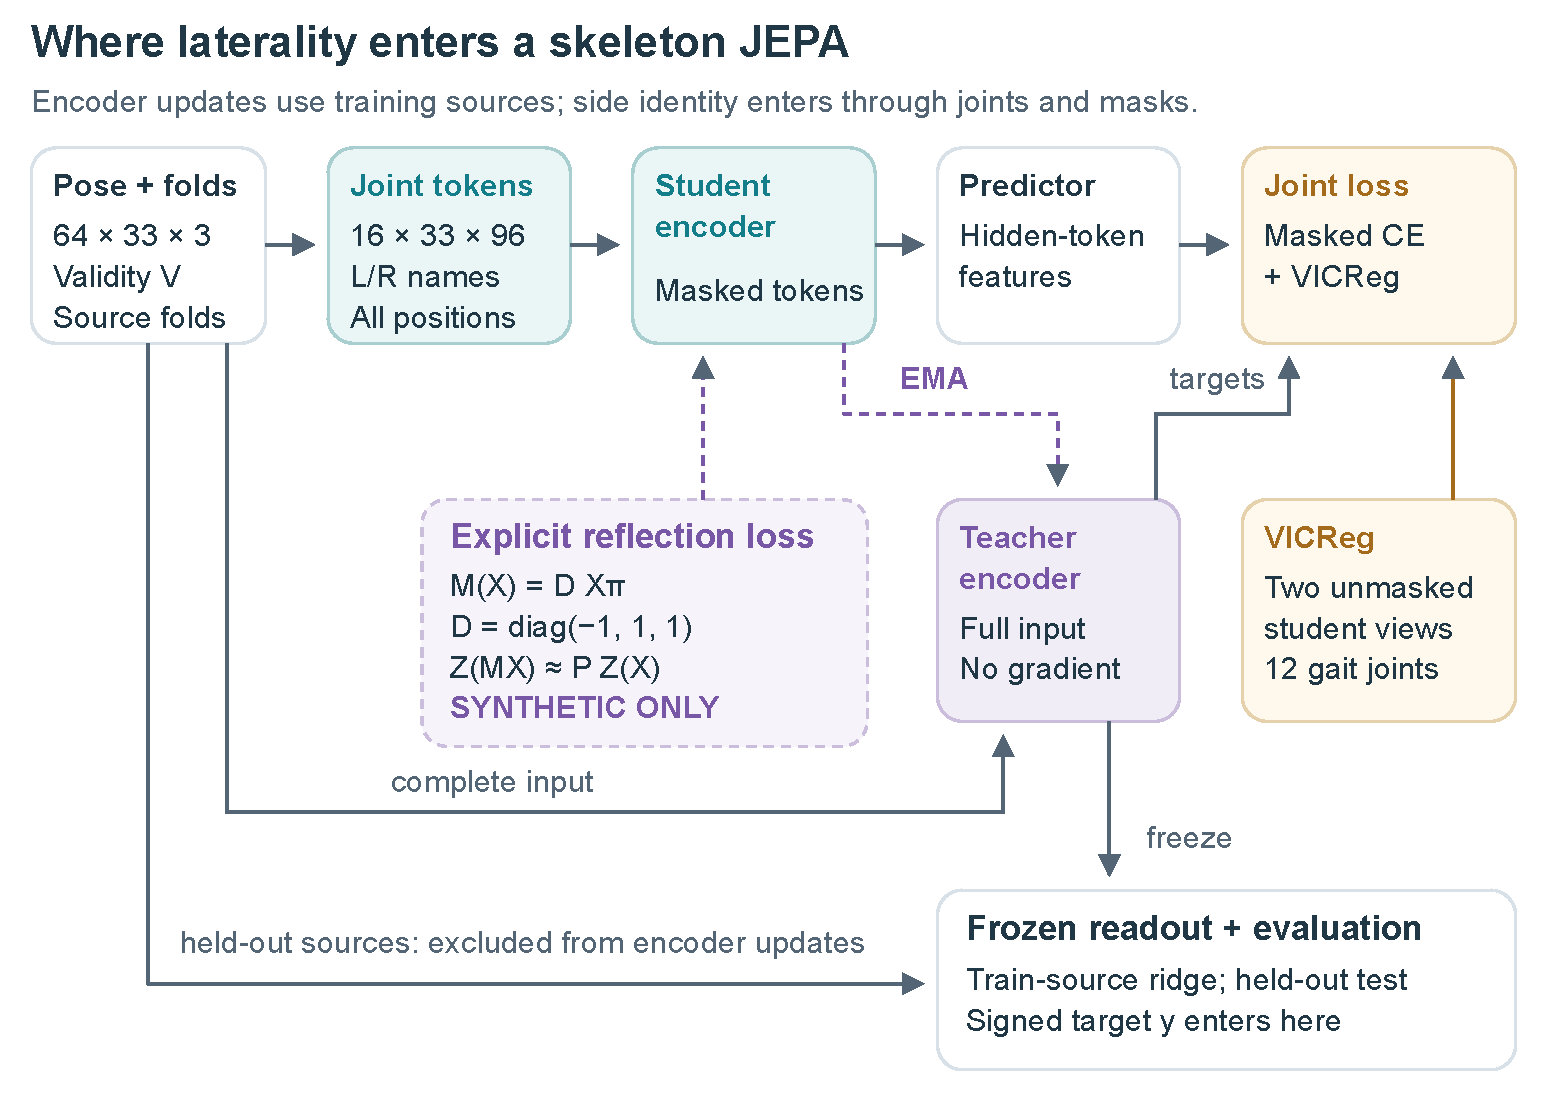
\includegraphics[width=\linewidth]{training_pipeline_compact_print.pdf}
\caption{Bilateral geometry enters through paired landmark identities, gait-based masking or pooling, and the optional reflection branch. The dotted branch adds an explicit token-reflection penalty to the online encoder and has synthetic evidence only. The signed target is used after pretraining by the frozen-feature readout. Clip-local preparation precedes source-fold creation; every training draw and transformed view inherits the source assignment.}\label{fig:training_pipeline_compact}
\end{figure}

Five outer folds hold out 19, 19, 19, 18 and 18 sources, containing 189, 182, 72, 77 and 105 clips. All clips, mirrors and augmentations from a video remain together. Each fold and seed starts a new encoder using only its outer-training sources; source-balanced sampling controls the contribution of videos with many clips. Four inner folds in the reflection study and three in the mask and motion-readout studies select ridge penalties. Ridge is linear regression with a penalty on coefficient size, used here to limit unstable fits to many features. Each imputer and scaler is fitted within the corresponding inner fitting partition, then refitted with the selected penalty on all outer-training sources. Inner validation selects the readout only: its unlabeled clips already entered that outer fold's encoder pretraining.

All completed real-data comparisons use 64 frames and 33 landmarks, width 96, encoder/predictor depths 4/2, four attention heads, batch size 20, and 1,200 updates. The online encoder retains the full token grid but zeros hidden coordinate embeddings before adding positions. The predictor estimates teacher distributions at hidden locations using cross-entropy. The teacher receives no gradients and follows an exponential moving average of online weights. An auxiliary VICReg \citep{ref14} loss, weighted by 0.05, regularizes agreement and feature variation over two unmasked geometric views pooled at twelve gait landmarks. Thus changing hidden-target eligibility does not remove all anatomical priors.

Paired arms share initialization, source draws, geometric views and update counts, with separate random streams for masking. Mask losses preserve each clip's own target indices and average within clip before averaging clips. Invalid targets do not contribute. The regularizer legitimately receives complete training views, so the masked prediction pathway is not the encoder's only exposure to those observations.

The reflection-augmentation condition mirrors training clips with probability 0.5. The motion and region mask conditions use neither reflection augmentation nor an explicit reflection penalty. A separate reflection-loss experiment uses unreflected and mirrored online-encoder passes, aligns anatomical tokens, and leaves feature channels unchanged. Its evidence is synthetic; Appendix B describes the loss and additional compute. None of these encoder objectives uses the signed target or an affected-side label.

\subsection{Evaluation and statistical inference}\label{evaluation-and-statistical-inference}

For \(V\) sources and \(n_v\) clips from source \(v\), each clip has weight \(w_{vi}=1/(Vn_v)\). With \(\bar y_w=\sum w_{vi}y_{vi}\), \[
R^2_w=1-\frac{\sum_{vi}w_{vi}(y_{vi}-\hat y_{vi})^2}
{\sum_{vi}w_{vi}(y_{vi}-\bar y_w)^2}.
\] Each source therefore receives equal total weight even when it supplies many clips. Within a seed, predictions from all five held-out folds are pooled before computing \(R^2\); the reported result averages the five seed-specific scores. It is neither an average of fold \(R^2\) values nor a score from an ensemble of seed-averaged predictions. Negative \(R^2\) means squared error exceeds variation around the weighted evaluation mean; a separately fitted training-source mean is the usable prediction baseline.

Scores and interval bounds are rounded from full-precision results to three decimal places, with differences computed before rounding. Nonzero differences smaller than 0.001 retain one significant digit so that rounding does not hide their sign.

Paired uncertainty resamples entire videos while retaining their clips and paired seed predictions. For a mask comparison the null is no positive difference in source-balanced readout performance relative to the count-matched random policy; for learning it is no positive difference relative to matched initialization. These are superiority questions, and no equivalence margin or power guarantee is established. The directly audited mask and trained-versus-initial contrasts use 2,000 resamples. Their intervals condition on the fitted models and exclude full-retraining and new-split uncertainty. The summary-only reflection comparison used a separate 2,000-resample analysis; its complete inputs remain unavailable. Repeated seeds and diagnostic mask draws are not independent participants. The same development cohort informed the full set of experiments, so source separation within each comparison does not make the whole study confirmatory.

\section{Results}\label{results}

\subsection{Measurement agreement and reflection}\label{measurement-agreement-and-reflection}

Recomputing the target on prepared input provides finite paired measurements for 623 clips from 92 sources. The source-weighted sign agreement with the original measurement is 70.4\%, and direct calculation-agreement \(R^2\) is 0.218. This descriptive check flags a mismatch in the measurement path. It neither localizes the responsible preparation step nor estimates a model's accuracy or information ceiling.

The reflection-augmentation comparison reports a small improvement in a normalized token discrepancy \(q\), which compares reflected teacher tokens with anatomically exchanged unreflected tokens while keeping feature channels unchanged. It shows no demonstrated corresponding gain in observable laterality, and both trained variants remain worse than initialization under that token action. Only summary results were available for this comparison, so its uncertainty analysis was not independently repeated.

This test fixes the feature-channel action to identity; failure does not rule out another learned reflection transformation. An algebraically odd output or constant nonzero token vector can also satisfy a symmetry criterion without useful movement prediction, as illustrated in Appendix B.

\subsection{Do different hidden targets improve the observable outcome?}\label{do-different-hidden-targets-improve-the-observable-outcome}

A matched-count comparison of gait-only and all-landmark scattered targets found no demonstrated advantage. The motion and region mask comparisons include 25 motion fold/seed jobs with three conditions each and 25 region jobs with two conditions each, totaling 125 encoders.

The motion-mask budget uses 0.5 of the smaller gait-derived pool, yielding an average of 80.8 targets, about 17\% of valid all-landmark tokens. It does not hide half the body grid. MAMP-style and robust motion weighting increase target-motion enrichment under the common audit statistic. Connected regions hide about 9.9\% of valid tokens, reducing the fraction of hidden targets with immediate visible time brackets from about 70\% to zero and with visible anatomical neighbors from about 99\% to 51\%. These are successful changes to selection and local context; they do not establish what the contextualized teacher features represent.

\begin{table}[htbp]
\centering
\small
\begin{tabular}{@{}
  >{\raggedright\arraybackslash}p{(\linewidth - 4\tabcolsep) * \real{0.4600}}
  >{\raggedleft\arraybackslash}p{(\linewidth - 4\tabcolsep) * \real{0.2200}}
  >{\raggedright\arraybackslash}p{(\linewidth - 4\tabcolsep) * \real{0.3200}}@{}}
\toprule\noalign{}
\begin{minipage}[b]{\linewidth}\raggedright
Alternative minus its own random reference
\end{minipage} & \begin{minipage}[b]{\linewidth}\raggedleft
\(\Delta R^2\)
\end{minipage} & \begin{minipage}[b]{\linewidth}\raggedright
95\% source interval
\end{minipage} \\
\midrule\noalign{}

MAMP-style motion weighting & −0.0008 & {[}−0.020, 0.015{]} \\
Robust motion mixture & 0.0005 & {[}−0.015, 0.015{]} \\
Connected region & −0.009 & {[}−0.033, 0.018{]} \\
\bottomrule
\end{tabular}
\end{table}

Each comparison covers 625 clips, 93 sources and five seeds. Motion and region families have different budgets and separate references. Their intervals allow small improvements or losses, establishing neither superiority nor equivalence. Whole trajectories and interior gaps have coverage audits but no completed training comparison. No mask is selected as best on these outer-test results.

\subsection{Does pretraining help when the readout retains more movement statistics?}\label{does-pretraining-help-when-the-readout-retains-more-movement-statistics}

A mean summary combines left-minus-right and left-plus-right feature means for five pairs, giving 960 features. Adding temporal standard deviations, mean absolute feature increments and ten support fractions gives 2,890. The latter improves the initial encoder from \(R^2=0.071\) to \(0.223\), while trained teachers reach only \(0.101\)--\(0.114\) under the same summary. Every trained arm has lower \(R^2\) and higher mean absolute error than its matched initial encoder in all five seeds. Final online encoders are also below initialization.

The term ``initial'' removes only S-JEPA pretraining. The control retains the learned pose detector, anatomical schema, preparation, engineered summary and supervised ridge fit. Its improved readout demonstrates access under that procedure. Temporal SD does not encode ordering, and support features can describe missingness; the change in feature count also affects supervised capacity and regularization.

We computed paired trained-minus-initial intervals from the saved predictions, without retraining. These exploratory, marginal intervals lie below zero for all five arms. For the motion-uniform reference, the \(R^2\) difference is \(-0.109\), with interval \([-0.170,-0.041]\). Appendix A gives all contrasts and the assumptions of the uncertainty analysis. This is evidence of a deficit for the tested learning/readout combination, rather than proof that all motion information was destroyed.

Ridge regularization remains unresolved: 39\% of teacher and 77\% of online fits using the enhanced summary select the largest candidate, 10,000. A wider common search and summary-component controls could change the estimates. The direct-pose summary gives \(R^2=0.035\); it is one linear-readout baseline, not the best possible use of the coordinates.

\subsection{What did the predictor learn?}\label{what-did-the-predictor-learn}

\begin{figure}[!tbp]
\centering
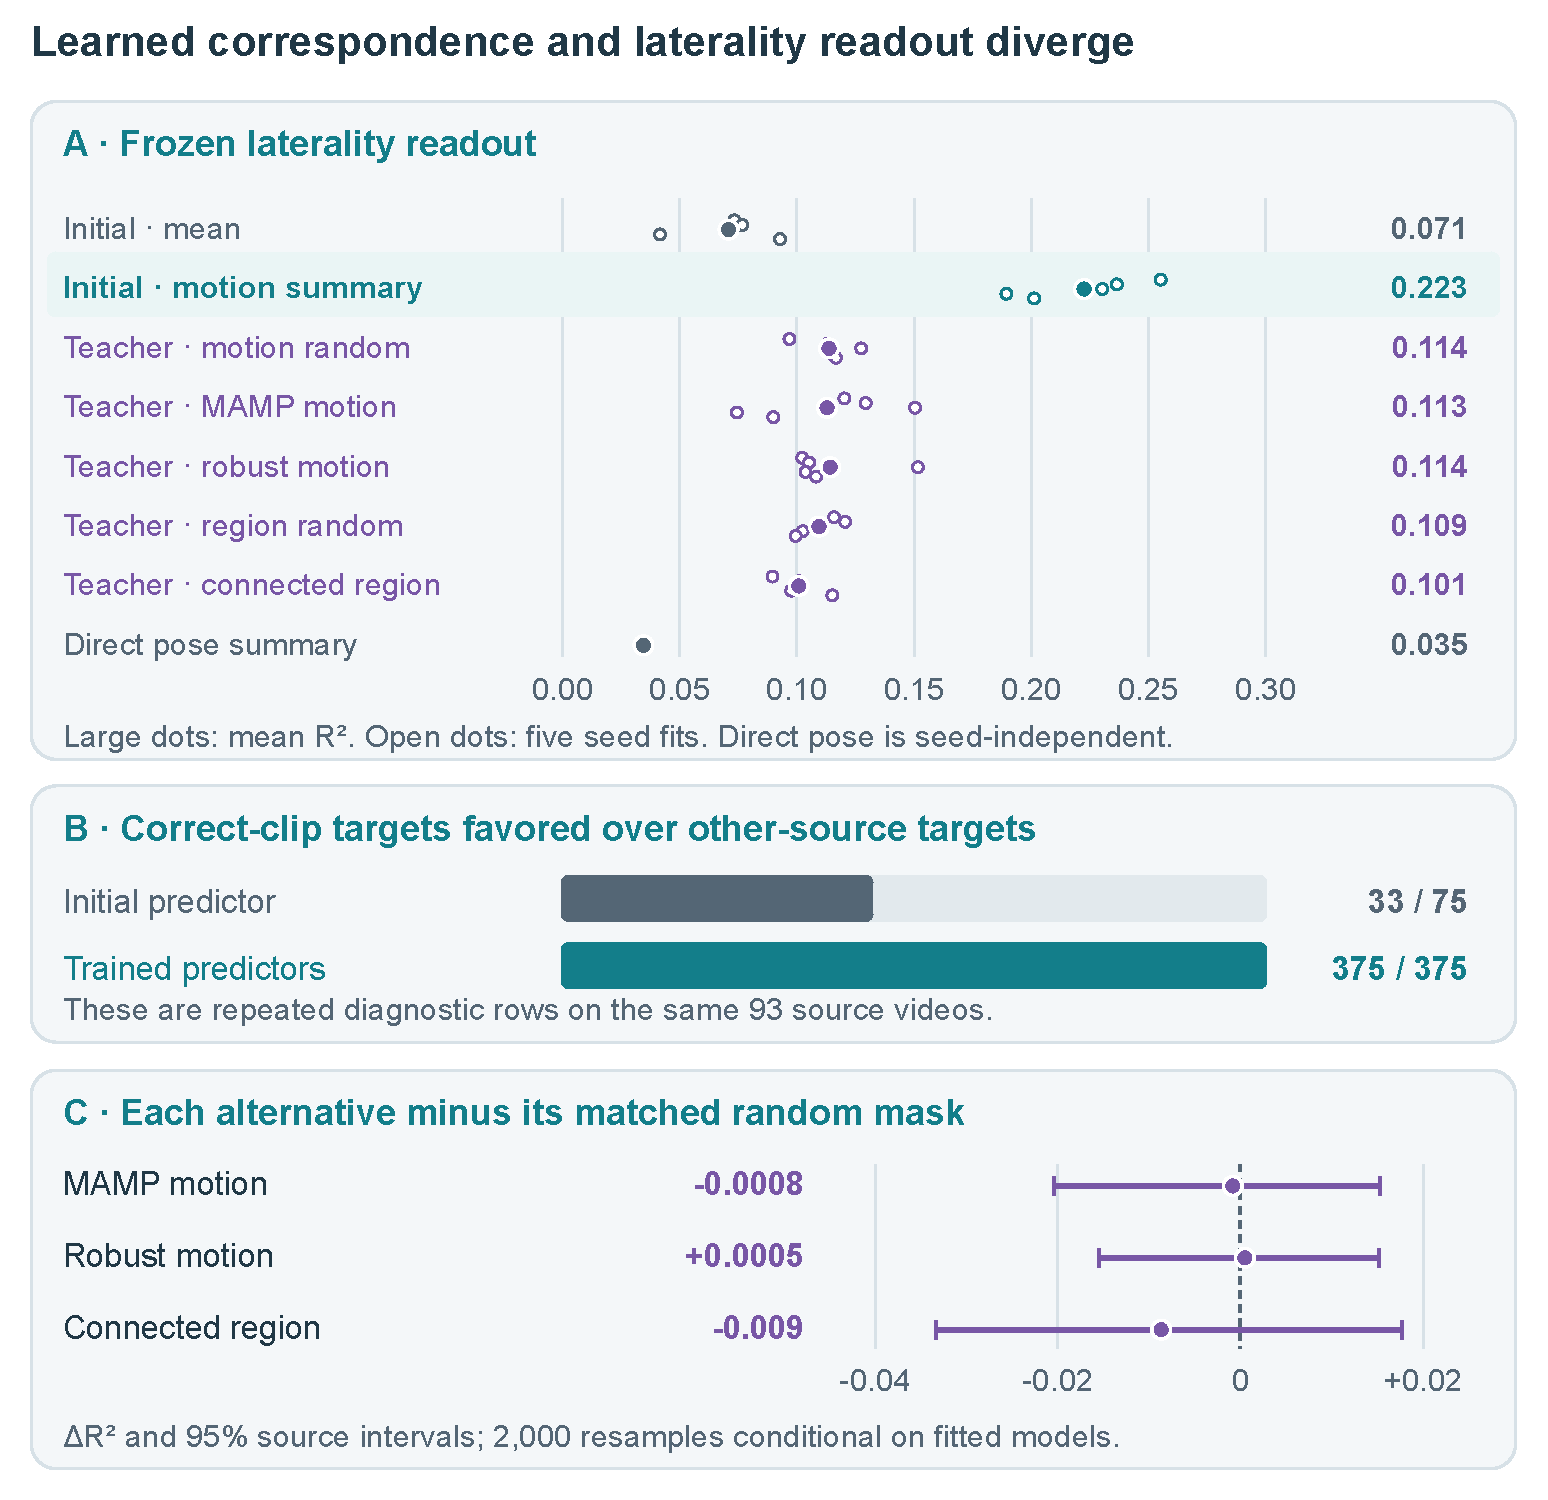
\includegraphics[width=\linewidth]{learning_results_print.pdf}
\caption{Predictors improve clip correspondence while their frozen encoders produce weaker laterality readouts than matched initialization. Seed points are repeated fits on the same 93 videos, not independent cohorts or confidence intervals. The 375 trained diagnostic rows are 125 fits evaluated under three masks; reused initial controls are deduplicated. Panel C contains the retained mask-versus-reference source-bootstrap intervals, distinct from Appendix A's new learning contrasts. All plotted values come from the directly audited saved grid.}\label{fig:learning_results}
\end{figure}

Every trained predictor diagnostic favors its correct clip's hidden teacher features over a valid mismatched target from another source, using the same control clips and positions. Initial controls do not show a consistent preference. Since the teacher features are contextualized using the full clip, this correspondence can depend on information already visible in the context. Static posture, viewpoint, support or motion may contribute; the diagnostic does not isolate recovery of withheld movement.

Each arm predicts its own teacher's feature distributions. A lower loss can accompany changed target variation, so neither raw cross-entropy nor between-arm feature-error magnitudes rank physical usefulness. The shared coordinate-derived endpoint provides the complementary evaluation. Recorded diagnostics do not establish complete feature collapse, and the present results do not identify the mechanism of the learned readout deficit.

\section{Discussion and a decisive next experiment}\label{discussion-and-a-decisive-next-experiment}

Bilateral geometry provides a common relation that can be followed from pose coordinates through masking, feature prediction, and frozen evaluation. That path reveals several distinct limitations. The target changes appreciably when it is recalculated after input preparation, so an early readout failure cannot be attributed to the encoder alone. Count-matched masking changes the selected motion and local context without a demonstrated laterality benefit. A richer readout helps the initial encoder much more than the trained representations, even though the trained predictors acquire correct-clip correspondence. The next question is therefore where information about the signed movement contrast becomes difficult to recover along the measurement, representation, and readout path.

The most economical follow-up uses saved encoders to isolate support fractions, match summary dimensions, expand ridge penalties, and compare target calculations after each preparation step. These tests would help distinguish changes in the measurement from limits of the representation or readout. A pilot used to choose a pretraining recipe must exclude its validation videos from that encoder's training, not only from its readout fit.

After fixing that evaluation, compare the same recipe with and without explicit reflection training. Success should require improved observable prediction over both the matched base recipe and initialization, the intended transformation behavior, and retained feature variation. A lower \(q\) alone would leave the central utility question open. Measure the extra encoder passes and keep failed outcomes. The results can guide that design, but a new source collection or independently specified setting is needed for stronger confirmation.

Future prediction would provide a more direct link to temporal world models. It requires strictly past-only inputs and common future-coordinate endpoints, compared with simple persistence and recent-velocity forecasts. A median speed contrast does not measure temporal direction, so even a successful laterality readout would be insufficient to validate a dynamics model. Our finding that clip-specific correspondence improves while bilateral movement becomes harder to recover motivates including observable geometric consequences in that evaluation. Real-data forecasts and recursive rollouts remain to be tested.

\section{Scope, ethics and reproducibility}\label{scope-ethics-and-reproducibility}

GAVD suits our question because its clinician-annotated normal and abnormal gait spans different movement patterns and recording conditions. The dataset paper \citep{ref13} describes ordinary RGB recordings from clinical and uncontrolled settings. This gives bilateral geometry a practical role in Physical World AI: paired landmark motion must be measured across recording viewpoints and with uncertain pose estimates. Walking intervals, bounding boxes and source identifiers support traceable pose extraction and grouping of clips by recording. The open annotations \citep{ref15} make this selection process accessible to other researchers. Clinical categories contextualize the movement diversity, while our coordinate-derived target permits evaluation without disease labels during encoder training.

These advantages support evaluation on our selected GAVD subset. Repeated people across videos cannot be ruled out. Clinical annotations describe observed gait, and our cohort provides no verified affected-side labels or independent validation of the signed contrast. The target omits temporal phase and loading and may cancel pairwise asymmetries. The study measures performance after the research plan was developed on excluded source videos; it establishes neither population representativeness nor multimodal sensing or calibrated 3D dynamics.

The repository's MIT License \citep{ref16}, copyright 2024 Rahmyyy, permits use, modification and redistribution of covered materials without a license fee, including research and commercial use. Copies or substantial portions must retain the copyright and permission notices; warranties and liability are disclaimed. The maintainers explicitly permit research use of the supplied annotations under this license \citep{ref15}. This openness enables others to inspect cohort definitions and adapt annotation-based workflows.

As stated in the access policy \citep{ref15}, the repository supplies annotations, metadata and YouTube links; original videos require independent retrieval under platform terms, institutional ethics requirements and applicable copyright and data-protection law. Repository licensing therefore does not establish redistribution rights for those videos or our derived poses. Link removal can also prevent reconstruction of the same cohort. Reproduction should record annotation versions, retrieval dates, exclusions and source splits. Our institutional ethics, data-use and derived-pose release reviews remain unresolved; documenting MIT does not complete those reviews.

We independently recomputed 200 pooled score rows and three saved mask intervals from 125,000 saved predictions, verified grid-table hashes and checked 125 complete update histories. Checkpoint predictions were not regenerated, and unavailable reports were not reproduced. The {core evidence record}, {extension evidence record}, {recomputation script} and {figure provenance} document this scope. These are internal manuscript artifacts; no submission or artifact release is authorized by this review.
\label{physworld:main-last}
\clearpage
\label{physworld:references-start}
{\renewcommand{\bibfont}{\small}
\begin{thebibliography}{99}
\bibitem{ref01} K. K. Patterson, I. Parafianowicz, C. J. Danells, V. Closson, M. C. Verrier, W. R. Staines, S. E. Black, and W. E. McIlroy. \href{https://pubmed.ncbi.nlm.nih.gov/18226655/}{Gait asymmetry in community-ambulating stroke survivors}. \emph{Archives of Physical Medicine and Rehabilitation}, 89(2):304--310, 2008. doi:10.1016/j.apmr.2007.08.142.

\bibitem{ref02} M. D. Lewek, R. Poole, J. Johnson, O. Halawa, and X. Huang. \href{https://pubmed.ncbi.nlm.nih.gov/19945285/}{Arm swing magnitude and asymmetry during gait in the early stages of Parkinson's disease}. \emph{Gait \& Posture}, 31(2):256--260, 2010. doi:10.1016/j.gaitpost.2009.10.013.

\bibitem{ref03} S. M. Brændvik, T. Goihl, R. S. Braaten, and B. Vereijken. \href{https://pubmed.ncbi.nlm.nih.gov/32082235/}{The Effect of Increased Gait Speed on Asymmetry and Variability in Children With Cerebral Palsy}. \emph{Frontiers in Neurology}, 10:1399, 2020. doi:10.3389/fneur.2019.01399.

\bibitem{ref04} I. Vandekerckhove, M. Van den Hauwe, N. De Beukelaer, E. Stoop, M. Goudriaan, M. Delporte, G. Molenberghs, A. Van Campenhout, L. De Waele, N. Goemans, F. De Groote, and K. Desloovere. \href{https://pmc.ncbi.nlm.nih.gov/articles/PMC9201072/}{Longitudinal Alterations in Gait Features in Growing Children With Duchenne Muscular Dystrophy}. \emph{Frontiers in Human Neuroscience}, 16:861136, 2022. doi:10.3389/fnhum.2022.861136.

\bibitem{ref05} M. Abdelfattah and A. Alahi. \href{https://www.ecva.net/papers/eccv_2024/papers_ECCV/papers/04755.pdf}{S-JEPA: A Joint Embedding Predictive Architecture for Skeletal Action Recognition}. In \emph{Computer Vision -- ECCV 2024}, volume 15090 of \emph{Lecture Notes in Computer Science}, pages 367--384. Springer, 2025. doi:10.1007/978-3-031-73411-3\_21.

\bibitem{ref06} Y. Mao, J. Deng, W. Zhou, Y. Fang, W. Ouyang, and H. Li. \href{https://arxiv.org/abs/2308.07092}{Masked Motion Predictors are Strong 3D Action Representation Learners}. In \emph{Proceedings of the IEEE/CVF International Conference on Computer Vision (ICCV)}, pages 10181--10191, 2023.

\bibitem{ref07} J. Do, Y. Chen, G. Youk, and M. Kim. \href{https://arxiv.org/abs/2603.10648}{Less is More: Compact-Token Masked Feature Prediction for Skeleton Representation Learning}. arXiv preprint arXiv:2603.10648v3, 2026.

\bibitem{ref08} H. Ghaemi, E. B. Muller, and S. Bakhtiari. \href{https://proceedings.neurips.cc/paper_files/paper/2025/hash/2f63d2963526bdd9ff1b8bcc2dc9905a-Abstract-Conference.html}{seq-JEPA: Autoregressive Predictive Learning of Invariant-Equivariant World Models}. In \emph{Advances in Neural Information Processing Systems}, volume 38, pages 32943--32973, 2025. doi:10.52202/085713-1104.

\bibitem{ref09} J. Lee, C. Kim, H. Kim, K. Lee, and J. Lee. \href{https://proceedings.iclr.cc/paper_files/paper/2026/hash/3be6511c8f56d0dca4b5ed59fdf9b2f4-Abstract-Conference.html}{Soft Equivariance Regularization for Invariant Self-Supervised Learning}. In \emph{Proceedings of the International Conference on Learning Representations (ICLR)}, pages 35502--35521, 2026.

\bibitem{ref10} L. Mur-Labadia, M. Muckley, A. Bar, M. Assran, K. Sinha, M. Rabbat, Y. LeCun, N. Ballas, and A. Bardes. \href{https://arxiv.org/abs/2603.14482}{V-JEPA 2.1: Unlocking Dense Features in Video Self-Supervised Learning}. arXiv preprint arXiv:2603.14482v3, 2026.

\bibitem{ref11} H. Wei, L. Sun, and G. Zhao. \href{https://arxiv.org/abs/2608.21160}{Human-JEPA: A Human-Centric Vision Model that Perceives and Anticipates}. arXiv preprint arXiv:2608.21160v1, 2026.

\bibitem{ref12} M. J. Marin-Jimenez, I. Jimenez-Velasco, and R. Muñoz-Salinas. \href{https://github.com/AVAuco/GaitJEPA}{GaitJEPA: How Far Can We Go with JEPA on Binary Silhouettes for Gait Recognition?} Accepted for the \emph{IEEE International Joint Conference on Biometrics (IJCB)}, 2026; author repository, accessed 10 September 2026.

\bibitem{ref13} R. Ranjan, D. Ahmedt-Aristizabal, M. A. Armin, and J. Kim. \href{https://arxiv.org/abs/2407.04190}{Computer Vision for Clinical Gait Analysis: A Gait Abnormality Video Dataset}. \emph{IEEE Access}, 13:45321--45339, 2025. doi:10.1109/ACCESS.2025.3545787.

\bibitem{ref14} A. Bardes, J. Ponce, and Y. LeCun. \href{https://arxiv.org/abs/2105.04906}{VICReg: Variance-Invariance-Covariance Regularization for Self-Supervised Learning}. In \emph{Proceedings of the International Conference on Learning Representations (ICLR)}, 2022.

\bibitem{ref15} Rahmyyy. \href{https://github.com/Rahmyyy/GAVD/blob/a87859c881603443f200bcd640663d2c3d7a8136/README.md}{GAVD repository documentation and dataset access policy}. GitHub, n.d. README at commit a87859c; accessed 10 September 2026.

\bibitem{ref16} Rahmyyy. \href{https://github.com/Rahmyyy/GAVD/blob/a87859c881603443f200bcd640663d2c3d7a8136/LICENSE}{GAVD MIT License}. GitHub, n.d. Copyright 2024 Rahmyyy; LICENSE at commit a87859c; accessed 10 September 2026.
\end{thebibliography}
}
\clearpage
\appendix
\label{physworld:appendix-start}
\section{Supporting comparisons and uncertainty}\label{appendix-a.-supporting-comparisons-and-uncertainty}

The table supplements Figure 2 with paired trained-minus-initial contrasts. Each compares a final teacher with its matched initial encoder using the same motion-sensitive summary and supervised readout procedure, across 625 clips from 93 source videos and five seeds.

\begin{table}[htbp]
\centering
\small
\begin{tabular}{@{}
  >{\raggedright\arraybackslash}p{(\linewidth - 4\tabcolsep) * \real{0.4600}}
  >{\raggedleft\arraybackslash}p{(\linewidth - 4\tabcolsep) * \real{0.2200}}
  >{\raggedright\arraybackslash}p{(\linewidth - 4\tabcolsep) * \real{0.3200}}@{}}
\toprule\noalign{}
\begin{minipage}[b]{\linewidth}\raggedright
Training arm
\end{minipage} & \begin{minipage}[b]{\linewidth}\raggedleft
Learned minus initial \(R^2\)
\end{minipage} & \begin{minipage}[b]{\linewidth}\raggedright
95\% source interval
\end{minipage} \\
\midrule\noalign{}

Motion uniform & −0.109 & {[}−0.170, −0.041{]} \\
MAMP-style motion & −0.110 & {[}−0.165, −0.051{]} \\
Robust motion & −0.108 & {[}−0.171, −0.042{]} \\
Region uniform & −0.113 & {[}−0.166, −0.060{]} \\
Connected region & −0.122 & {[}−0.183, −0.055{]} \\
\bottomrule
\end{tabular}
\end{table}

These exploratory intervals use 2,000 paired resamples of whole source videos, retaining clips and seed predictions together. They condition on fitted models and existing source splits, exclude retraining uncertainty, and have no adjustment for multiple comparisons. Seeds repeat model fitting on the same cohort. All intervals lie below zero, supporting a deficit for the tested learning and readout procedure; a different, properly selected readout could change that conclusion.

\section{Measurement and training conventions}\label{appendix-b.-measurement-and-training-conventions}

Target speeds use original timestamps and transitions observed for both paired landmarks. Pelvis centering requires both hips; body scale uses the median valid shoulder-pair and hip-pair widths, with a unit fallback when unavailable. The contrast uses \(\epsilon=10^{-8}\). Model inputs separately interpolate short gaps, allow a median-pelvis fallback, and resample to 64 positions. These choices explain why a target recalculated from prepared inputs can differ from the original measurement. All 33 landmark identities remain allocated throughout training.

The retained cohort contains 270 normal, 183 myopathic, 75 stroke, 58 cerebral-palsy and 39 Parkinson's clips. These observational categories contextualize the selected sample; they do not specify the affected side or establish disease prevalence.

The training recipe uses AdamW with learning rate \(10^{-3}\), weight decay 0.05, gradient clipping at 1 and teacher EMA 0.999. Student/teacher temperatures are 0.10/0.06, with target-center EMA 0.9. Paired masking comparisons share source draws, initialization and update counts, while matching realized target counts within each clip.

The optional reflection term compares original and mirrored online-encoder tokens after joint exchange, with feature channels unchanged. For each clip, it divides squared token error over common valid positions by the combined feature energy on those positions, held fixed when calculating gradients and bounded away from zero; the loss then averages clips. Both branches receive gradients through two additional full-input passes. This term has synthetic evidence only; it was absent from the completed GAVD masking comparisons.

\begin{figure}[!tbp]
\centering
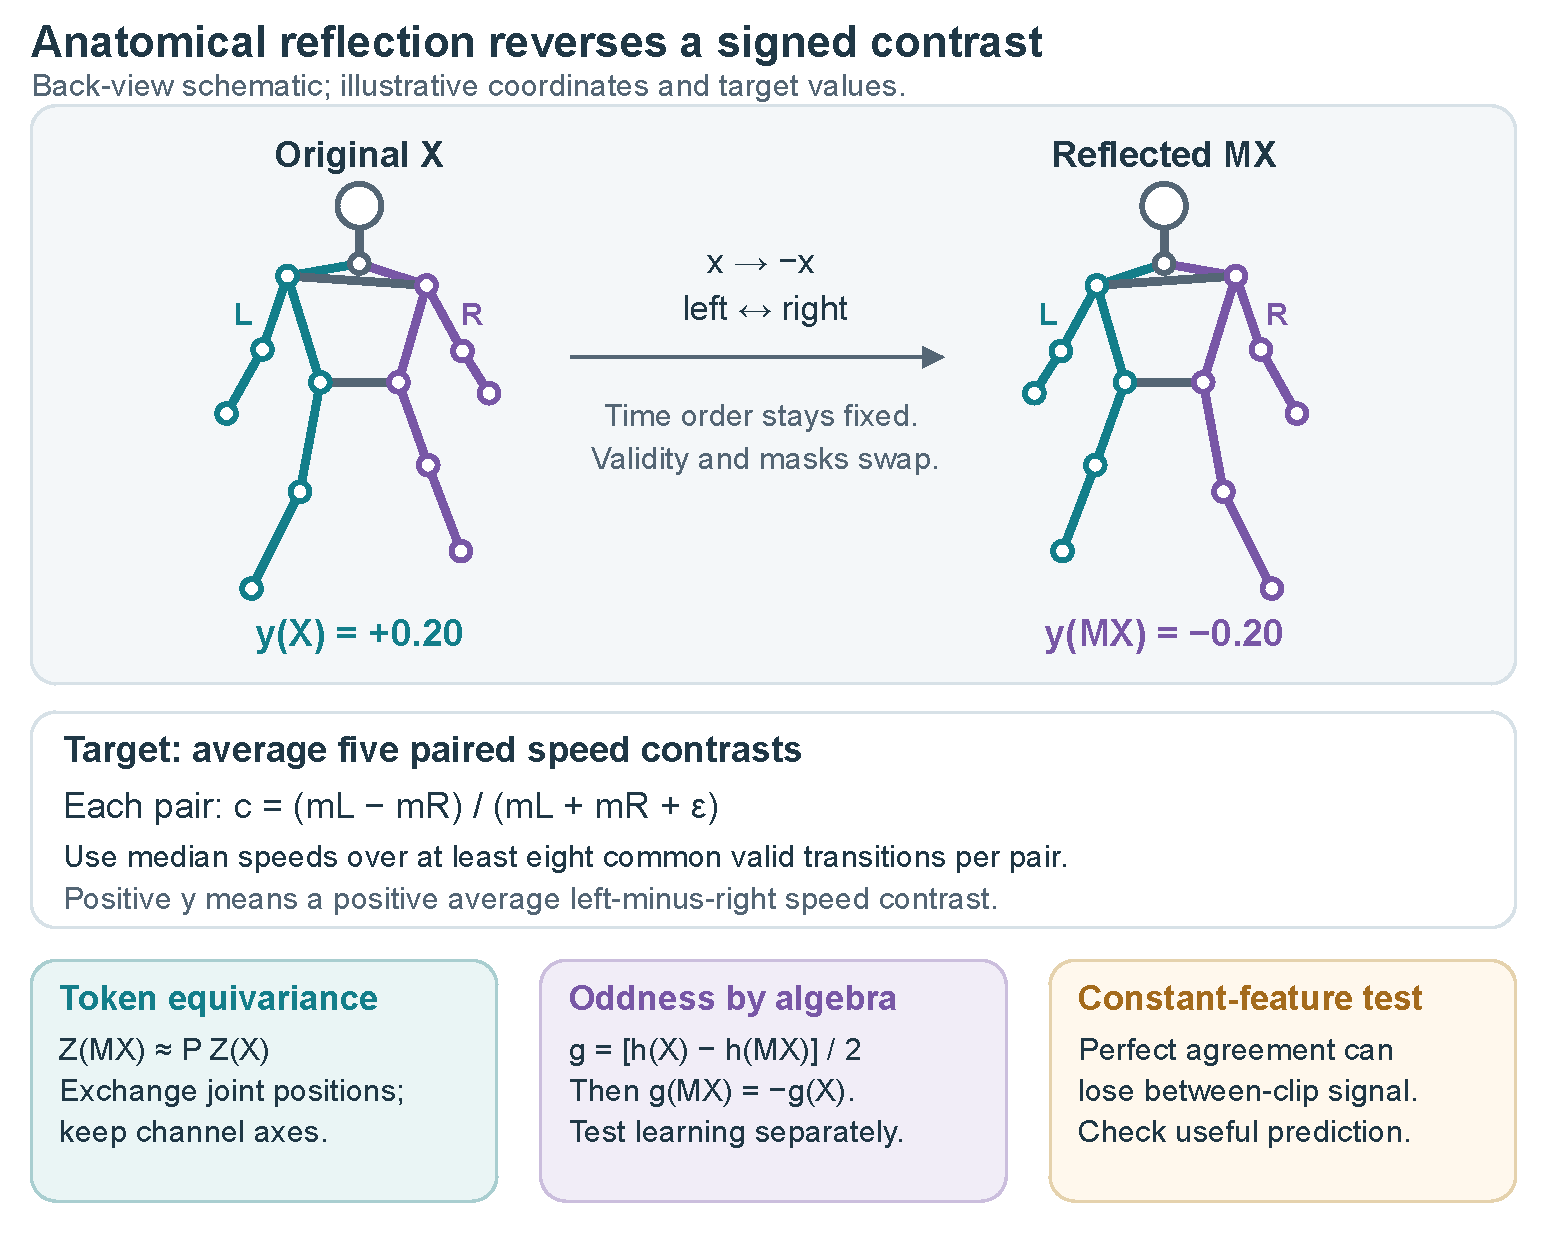
\includegraphics[width=\linewidth]{reflection_and_target_print.pdf}
\caption{Reflection exchanges anatomical sides and reverses the defined movement contrast. The lower panels show two controls: output symmetry can be imposed algebraically, and constant features can satisfy token consistency. Neither establishes accurate movement prediction. The bodies and values are schematic, with no participant measurements or clinical examples.}\label{fig:reflection_and_target}
\end{figure}
\end{document}
